% fig-blob.tex: the sealed vault as stored, one horizontal strip of fields (draft of 6 Nov 2026, at Cecil's mark in 4.3).
% Build from this folder:  pdflatex fig-blob.tex
% Source: Table 4.1 (the fields and their sizes) and the paragraph under it (the label, the fingerprint), section 4.3.
% Not to scale: the ciphertext is as long as the vault text.
\documentclass[tikz,border=4pt,11pt]{standalone}
% style.tex: what the four diagrams share (colours, fonts, the look of a party, a message, a note).
% The one accent colour is the blue of the latency charts; it always means "the head", the thing this thesis adds.
% Everything else is black or grey, so the figures still read when printed in black and white.
\usepackage[T1]{fontenc}
\usepackage{mathptmx}
\usetikzlibrary{positioning,calc,arrows,fit,backgrounds}
\definecolor{head}{HTML}{2A78D6}
\definecolor{ink}{HTML}{0B0B0B}
\definecolor{inktwo}{HTML}{52514E}
\definecolor{soft}{HTML}{F0EFEC}
\definecolor{rule}{HTML}{C3C2B7}
\tikzset{
  every picture/.style={font=\small, >=latex},
  party/.style={draw=ink, fill=soft, rounded corners=2pt, minimum width=3.4cm, minimum height=0.8cm, align=center, font=\small\bfseries},
  box/.style={draw=ink, fill=soft, rounded corners=2pt, minimum width=3.9cm, minimum height=1.9cm, align=center},
  quiet/.style={draw=rule, text=inktwo},
  life/.style={draw=rule, line width=0.9pt},
  msg/.style={->, draw=ink, line width=0.7pt},
  rep/.style={->, draw=ink, line width=0.7pt, dashed},
  hmsg/.style={->, draw=head, line width=1.2pt},
  hrep/.style={->, draw=head, line width=1.2pt, dashed},
  bad/.style={->, draw=ink, line width=1.2pt, dashed},
  lab/.style={font=\footnotesize, inner sep=3pt, text=ink},
  act/.style={font=\footnotesize, align=left, text=ink, fill=white, draw=rule, rounded corners=1.5pt, inner sep=3pt},
  outcome/.style={font=\footnotesize, align=center, text=ink, fill=white, draw=ink, rounded corners=1.5pt, inner sep=4pt},
  side/.style={font=\footnotesize\itshape, align=left, text=inktwo},
  band/.style={fill=soft, draw=rule, rounded corners=2pt, minimum height=0.7cm, font=\footnotesize, text=inktwo},
  holds/.style={font=\footnotesize, text=inktwo, fill=white, draw=rule, rounded corners=1.5pt, inner sep=2.5pt},
}

\usetikzlibrary{decorations.pathreplacing}
\tikzset{
  field/.style={draw=ink, fill=soft, minimum height=1.25cm, align=center, inner sep=2pt, font=\footnotesize},
  brace/.style={decorate, decoration={brace, amplitude=5pt}, draw=ink, line width=0.6pt},
  bracedown/.style={decorate, decoration={brace, amplitude=5pt, mirror}, draw=ink, line width=0.6pt},
  note/.style={font=\footnotesize, align=center, text=ink},
}
\begin{document}
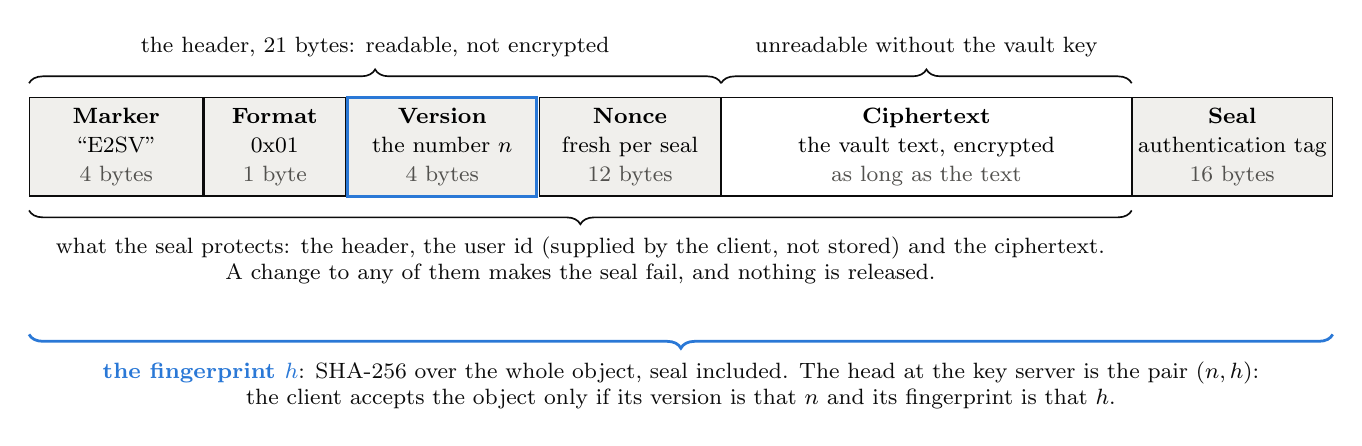
\begin{tikzpicture}
% ---------------------------------------------------------------- the strip
\node[field, minimum width=2.2cm, anchor=west] (magic) at (0,0) {\textbf{Marker}\\[1pt]``E2SV''\\[1pt]\textcolor{inktwo}{4 bytes}};
\node[field, minimum width=1.8cm, anchor=west] (fmt)   at (magic.east) {\textbf{Format}\\[1pt]0x01\\[1pt]\textcolor{inktwo}{1 byte}};
\node[field, minimum width=2.4cm, anchor=west, draw=head, line width=1.1pt] (ver) at (fmt.east) {\textbf{Version}\\[1pt]the number $n$\\[1pt]\textcolor{inktwo}{4 bytes}};
\node[field, minimum width=2.3cm, anchor=west] (nonce) at ([xshift=0.25pt]ver.east) {\textbf{Nonce}\\[1pt]fresh per seal\\[1pt]\textcolor{inktwo}{12 bytes}};
\node[field, minimum width=5.2cm, anchor=west, fill=white] (ct) at (nonce.east) {\textbf{Ciphertext}\\[1pt]the vault text, encrypted\\[1pt]\textcolor{inktwo}{as long as the text}};
\node[field, minimum width=2.2cm, anchor=west] (seal)  at (ct.east) {\textbf{Seal}\\[1pt]authentication tag\\[1pt]\textcolor{inktwo}{16 bytes}};
% ---------------------------------------------------------------- above: what is readable, what is not
\draw[brace] ([yshift=5pt]magic.north west) -- node[note, above=6pt] {the header, 21 bytes: readable, not encrypted} ([yshift=5pt]nonce.north east);
\draw[brace] ([yshift=5pt]ct.north west) -- node[note, above=6pt] {unreadable without the vault key} ([yshift=5pt]ct.north east);
% ---------------------------------------------------------------- below: what the seal protects
\draw[bracedown] ([yshift=-5pt]magic.south west) -- node[note, below=6pt] (sealtxt) {what the seal protects: the header, the user id (supplied by the client, not stored) and the ciphertext.\\ A change to any of them makes the seal fail, and nothing is released.} ([yshift=-5pt]ct.south east);
% ---------------------------------------------------------------- below: what the fingerprint covers (the head)
\draw[bracedown, draw=head, line width=1.0pt] ([yshift=-1.75cm]magic.south west) -- node[note, below=6pt] {\textcolor{head}{\textbf{the fingerprint $h$}}: SHA-256 over the whole object, seal included. The head at the key server is the pair $(n, h)$:\\ the client accepts the object only if its version is that $n$ and its fingerprint is that $h$.} ([yshift=-1.75cm]seal.south east);
\end{tikzpicture}
\end{document}
